\documentclass[conference]{IEEEtran}
\usepackage{enumitem}
\usepackage[document]{ragged2e}
\usepackage{blindtext}
\usepackage{graphicx}
\usepackage{float}
\usepackage{amsmath}
%\usepackage{natbib}
\usepackage{cite}

\graphicspath{ {./}{./images/} }

\title{Joint Radar Communication System using OFDM}

\author{

\IEEEauthorblockN{Owen Sowatzke}
\IEEEauthorblockA{\textit{Electrical Engineering Department} \\
\textit{University of Arizona}\\
Tucson, USA \\
osowatzke@arizona.edu}

\and
\IEEEauthorblockN{Iman Miraki}
\IEEEauthorblockA{\textit{Electrical Engineering Department} \\
\textit{University of Arizona}\\
Tucson, USA \\
imanmiraki@arizona.edu}}

\begin{document}
	\raggedbottom
	\maketitle
\section {Introduction}
     Vehicle-to-Vehicle (V2V) networks seek to enhance road safety and reduce traffic congestion by sharing road and traffic information between vehicles in real time. To avoid delays associated with third party networks, vehicle-to-vehicle communication systems need dedicated bandwidth. Instead of wasting additional spectrum resources, joint radar communication (JRC) systems attempt to integrate radar and communication systems. This results in reduced bandwidth usage and reduced power consumption while eliminating the need for additional hardware.
     
     In this paper, we design a JRC system, which uses OFDM for communication and zero-forcing to generate a range response from the OFDM returns. Next, we examine the performance of this system and compare it to standalone radar and standalone OFDM implementations.
        
  \section {Radar}
   \subsection {Background}
   
In this section, we provide background on frequency-modulated continuous wave (FMCW) radar, which is used in many automotive applications. FMCW radar continuously transmits a signal whose frequency varies linearly over time (chirp). It measures the time delay between the transmitted and the reflected signals (echoes) to determine the distance of reflecting objects. It can also determine the relative velocity of these objects, by measuring frequency shifts caused by the doppler effect.

	\begin{figure}[H]
    		\centering
    		\fbox{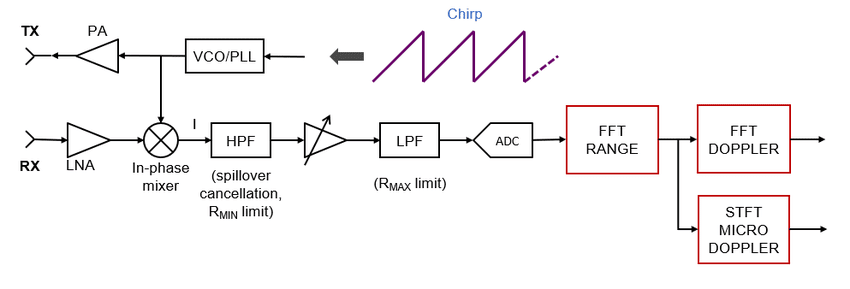
\includegraphics[width=0.9\linewidth]{FMCW Blockdiagram}}
    		\caption{Typical FMCW Block Diagram \cite{9613183}}
    		\label{fig::fmcw_radar}
	\end{figure}
	
 The block diagram shown in Figure \ref{fig::fmcw_radar} depicts the signal processing chain of a typical FMCW radar system. The transmitter generates a frequency-modulated chirp signal of the following form:
 
 	\begin{equation}
 		x(t) = e^{j\pi{\beta}t^2/\tau}
 		\label{eq::chirp}
 	\end{equation}
 	
 	where $\beta$ is the chirp bandwidth and $\tau$ is the chirp duration.
 	
	It transmits this signal out of the antenna towards objects of interest. The receiver receives reflections from each of these objects, which are passed through a low noise amplifier. For each return, the received signal will be a chirp waveform with a frequency offset as illustrated below.
	
	\begin{equation}
		r(t) = e^{j\pi{\beta}(t - t_0)^2/\tau} = e^{j\pi{\beta}t^2/\tau}e^{-j2\pi({\beta}t_0/\tau)t}e^{j\pi{\beta}t_0^2/\tau}
		\label{eq::delayed_chirp}
	\end{equation}
	
	We can mix the received signal with the transmitted signal to create a tone for each return. The frequency of this tone will be proportional to its delay.
	
	\begin{equation}
		f = \frac{{\beta}t_0}{\tau} \Rightarrow t_0 = \frac{{\tau}f}{\beta}
	\end{equation}
	
	The delay of this return is then related to the range of the reflecting object as follows:
	
	\begin{equation}
		R = \frac{ct_0}{2}
	\end{equation}
	
	The relationship between the transmitted and received chirps signals is illustrated below:
	
	\begin{figure}[H]
    		\centering
    		\fbox{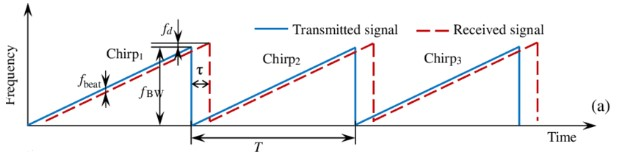
\includegraphics[width=0.8\linewidth]{FMCW Freq-Time graph}}
    		\caption{Plot of Transmit and Receive Signal Frequency vs Time.\cite{Long2019AssistingTV}}
    		\label{fig::fmcw_spectrogram}
	\end{figure}
	
	Note that the chirp bandwidth $\beta$ given in Equation (\ref{eq::chirp}) is inversely proportional to the range resolution ${\Delta}R$.
	
	\begin{equation}
		{\Delta}R = \frac{c}{2\beta}
		\label{eq::range_resolution}
	\end{equation}
	
	Because fine range resolution is desired, $\beta$ is typically very large (on the order of 150MHz-500MHz). This would typically require very high sample rates. However, one of the benefits of an FMCW radar is that the ADC samples tones instead of a full bandwidth signal. Thus, we only need to sample at a rate high enough to capture returns at the largest range of interest. For an automotive radar, this may only be on the order of 100-200 m, which can significantly reduce the sample rates and in turn reduce the radar's cost.
	
	After low-pass filtering and sampling the signal, Figure \ref{fig::fmcw_radar} illustrates the next step in the signal processing (a fast-time FFT). This FFT detects the frequency of each tone, which is proportional to the object's distance. Thus, the fast-time FFT allows the radar to detect the distance of reflecting objects.
	
	The object's relative velocity results in a doppler shift:
	
	\begin{equation}
		f_D = \frac{2v}{\lambda}
	\end{equation}
	
	Note that this doppler shift is twice what it is for a communication system, due to the reflection's two-way path. The phase change due to the doppler shift is small during a single chirp, so we instead measure it over multiple chirps (pulses). This is done by taking a slow-time FFT across pulses as shown in Figure \ref{fig::fmcw_radar}.
	
	The rate at which chirps (pulses) are repeated is denoted as the PRF. The PRF limits the radar's unambiguous range $R_{ua}$ and unambiguous velocity $v_{ua}$.
	
	\begin{equation}
		R_{ua} = \frac{c}{2\cdot\text{PRF}}
		\label{eq::unambig_range}
	\end{equation}
	
	\begin{equation}
		v_{ua} = \frac{\lambda\cdot\text{PRF}}{4}
		\label{eq::unambig_velocity}
	\end{equation}
	
	If a return exceeds these limits, it will alias and be detected at another range or velocity.
	
	\subsection {Simulation and Performance}

In this section, we evaluate the performance of an FMCW radar written in MATLAB and configured with the following set of parameters:

	\begin{center}
	\begin{tabular}{|c|c|}
		\hline
		Parameter & Value \\
		\hline
		Carrier Frequency & 77 GHz \\
		\hline
		Sample Rate & 300 MHz \\
		\hline
		PRF & 200 kHz \\
		\hline
		Number of Pulses & 256 \\
		\hline	
	\end{tabular}
	\end{center}
	
	Metrics of interest include the range resolution, peak sidelobe ratio (PSLR), doppler tolerance, unambiguous range, unambiguous velocity, and received SNR.

	The range resolution is the minimum range separation required for the radar to distinguish two objects. We can compute it according to Equation (\ref{eq::range_resolution}) as:
	
	\begin{equation}
		{\Delta}R = 0.5 m
	\end{equation}
	
	We can measure the range resolution by placing two objects very close together and observing the range response. In Figure \ref{fig::range_resolution}, we show the range response of two objects separated by 1 m. 
	 
	\begin{figure}[H]
	    	\centering
	    	\fbox{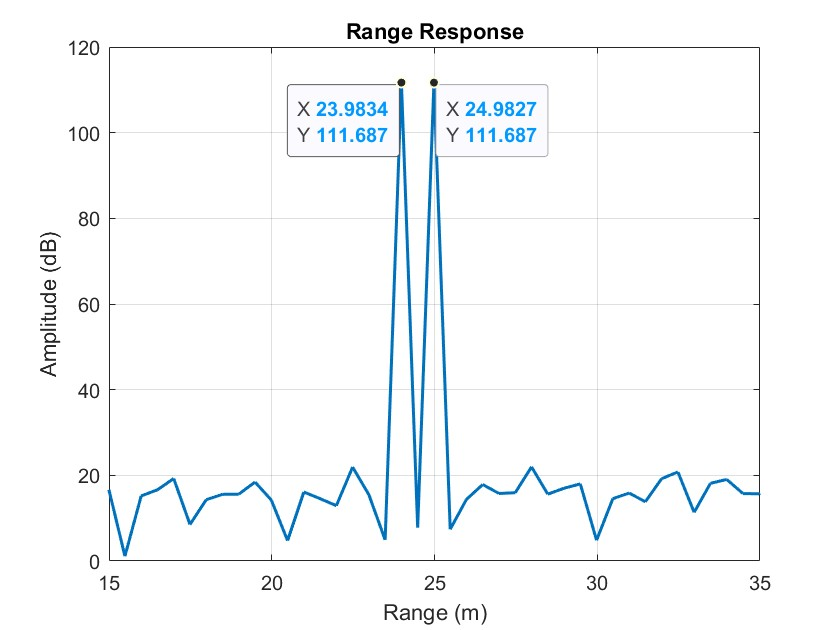
\includegraphics[width=0.8\linewidth]{range_resolution.jpg}}
	    	\caption{Range Response of Two Closely Placed Targets}
	    	\label{fig::range_resolution}
	\end{figure}
		
	Clearly, the minimum range separation at which the radar can distinguish two objects is when the objects are separated by a single range gate. This implies a range resolution of 0.5 m. This is consistent with the theoretical range resolution.
	
	The peak sidelobe ratio (PSLR) is the ratio of the range response peak to its highest sidelobe. The range response of an FMCW radar is the FFT of a tone (i.e. a sinc function). Therefore, the PSLR can vary drastically with the location of the FFT samples. To get a more consistent PSLR measurement, we zero-pad the fast-time FFT. Doing so, results in the following range response:
	
	\begin{figure}[H]
	    	\centering
	    	\fbox{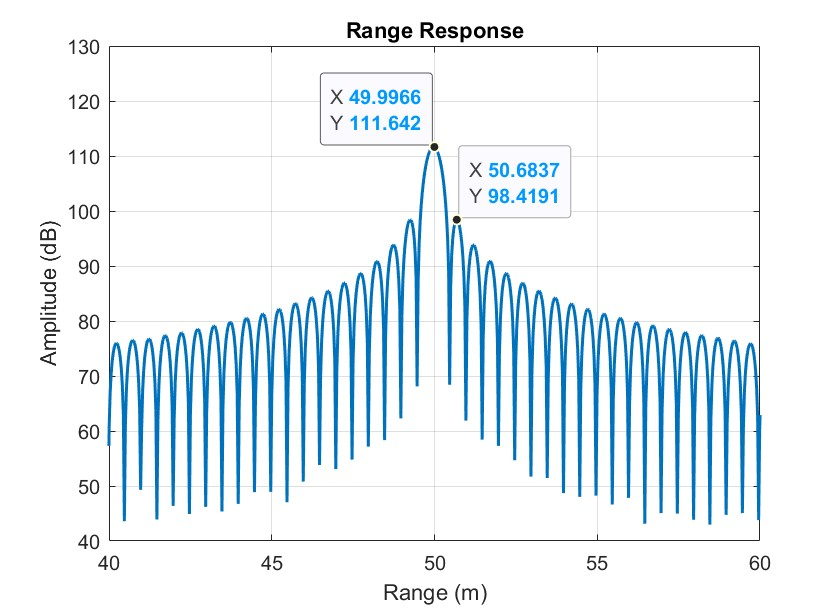
\includegraphics[width=0.8\linewidth]{pslr_no_window_zpad.jpg}}
	    	\caption{PSLR Measurement with Zero Padding in Fast-Time FFT}
	    	\label{fig::pslr_zpad}
	\end{figure}
	
	Examining the figure, we measure a PSLR of 13.27 dB, which is the expected PSLR measurement for a sinc function.
	
	Note that we can improve the PSLR by applying a window. However, this will also degrade the range resolution by increasing the range response's mainlobe width. First, we consider a Chebyshev window with an 80dB peak to sidelobe ratio. The resulting range response is shown in Figure \ref{fig::plsr_window}.
	
	\begin{figure}[H]
	    	\centering
	    	\fbox{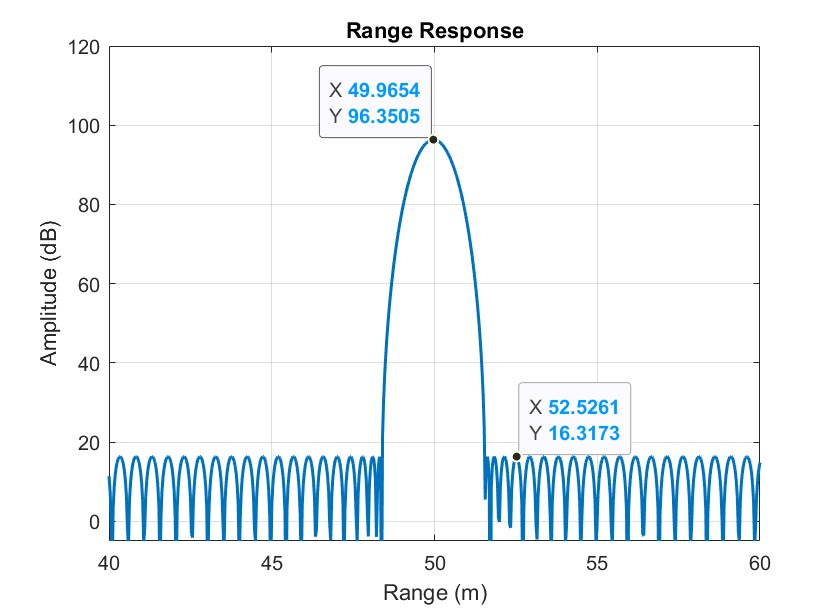
\includegraphics[width=0.8\linewidth]{pslr_with_window.jpg}}
	    	\caption{PSLR Measurement with Chebyshev Window}
	    	\label{fig::plsr_window} 
	\end{figure}
	
	Examining the range response, we achieve the expected PSLR of 80 dB. However, the mainlobe width is also increased by a factor of 3.2, which in term degrades the range resolution by a factor of 3.2. Other windows can be selected, which may off a better trade-off between range resolution and PSLR. Consider a taylor window, for example. It achieves a PSLR of 30.44 dB while only degrading the range resolution by a factor of 1.5.
	
	\begin{figure}[H]
	    	\centering
	    	\fbox{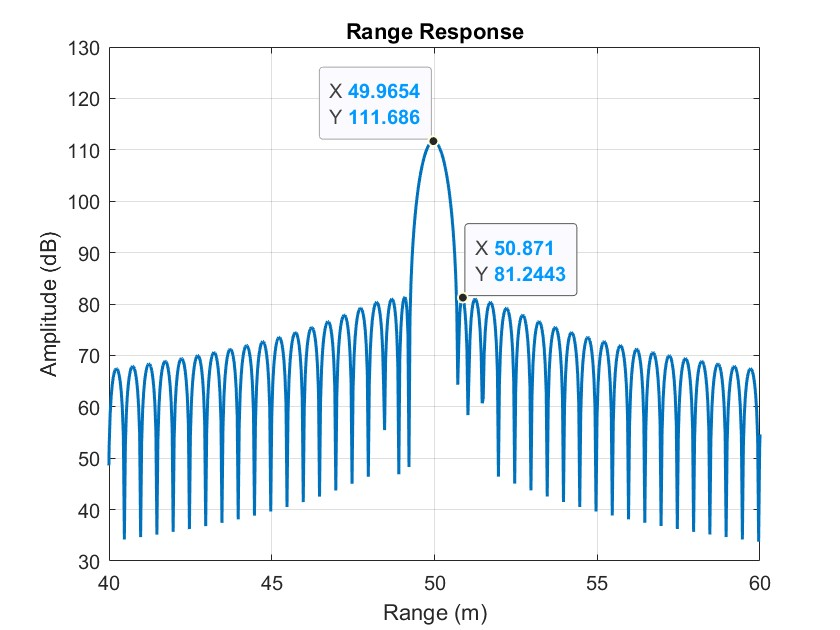
\includegraphics[width=0.8\linewidth]{pslr_with_taylor_window.jpg}}
	    	\caption{PSLR Measurement with Taylor Window}
	    	\label{fig::plsr_taylor_window} 
	\end{figure}
	
	We can measure the doppler tolerance of the system, by examining the PSLR in the presence of uncompensated doppler. In Figure \ref{fig::doppler_tolerance}, we show the PSLR when an 80 dB Chebyshev window is applied while sweeping the uncompensated doppler from $-v_{ua}$ to $v_{ua}$.
	
	\begin{figure}[H]
		\centering
	    	\fbox{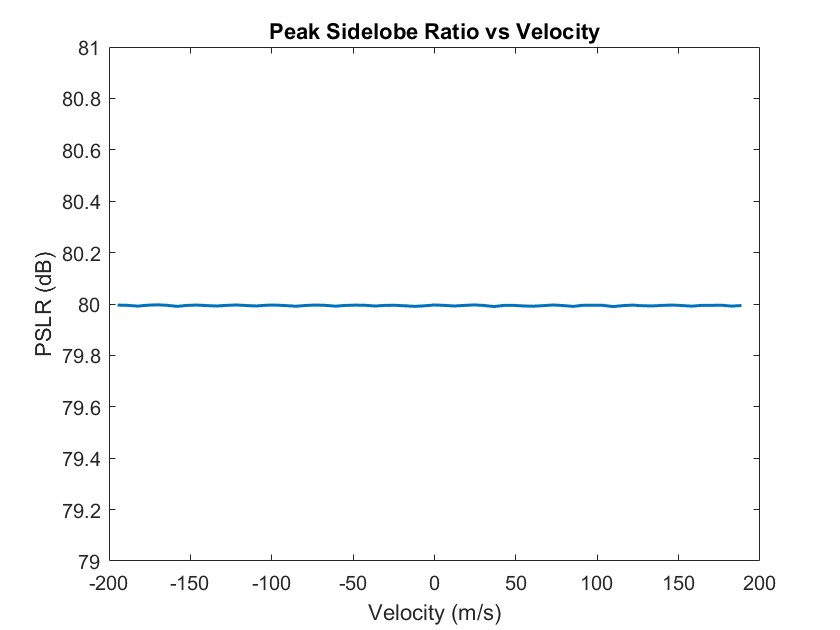
\includegraphics[width=0.8\linewidth]{doppler_tolerance.jpg}}
	    	\caption{PSLR Measurement with Uncompensated Doppler}
	    	\label{fig::doppler_tolerance} 
	\end{figure}
	
	Note that the PSLR is independent of the uncompensated doppler. This is because the uncompensated doppler simply adds to the frequency of the input tone. This can introduce range error through a process known as range-doppler coupling. However, as long as the doppler shift is in the first ambiguity, we can compensate for any introduced range error.
	
	The unambiguous range and velocity of the system can be computed according to Equation (\ref{eq::unambig_range}) and Equation (\ref{eq::unambig_velocity}). This results in the following:
	
	\begin{equation}
		R_{ua} = 750\ \text{m}
	\end{equation}
	
	\begin{equation}
		v_{ua} \approx 194.8\ \text{m/s}
	\end{equation}
	
	We can measure the ambiguous range and velocity by placing a reflecting object at ranges and velocities that exceed these limits. For instance, to measure the unambiguous range, we place an object at a range of 1250 m and examine the resulting range doppler matrix (RDM).
	
	\begin{figure}[H]
	    	\centering
	    	\fbox{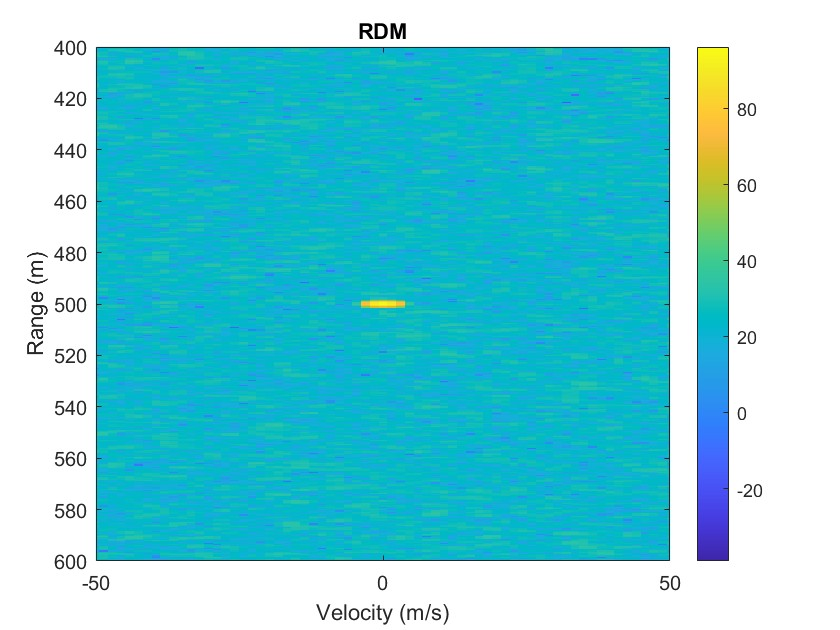
\includegraphics[width=0.8\linewidth]{ambig_range.jpg}}
	    	\caption{Range Doppler Matrix for Object at Ambiguous Range}
	    	\label{fig::ambig_range} 
	\end{figure}
	
	Figure \ref{fig::ambig_range} shows the RDM for this ambiguous range. The radar measures a range of 500.15 m. For an ideal system, the measured range is given as follows:
	
	\begin{equation}
		R_m = R\ \text{mod}\ R_{ua}
	\end{equation}
	
	Our measured range is consistent with this result thereby confirming the theoretical unambiguous range.
	
	We can confirm the unambiguous velocity in a similar manner. To do so, we measure the velocity of an object traveling at 250 m/s.
	
	\begin{figure}[H]
	    	\centering
	    	\fbox{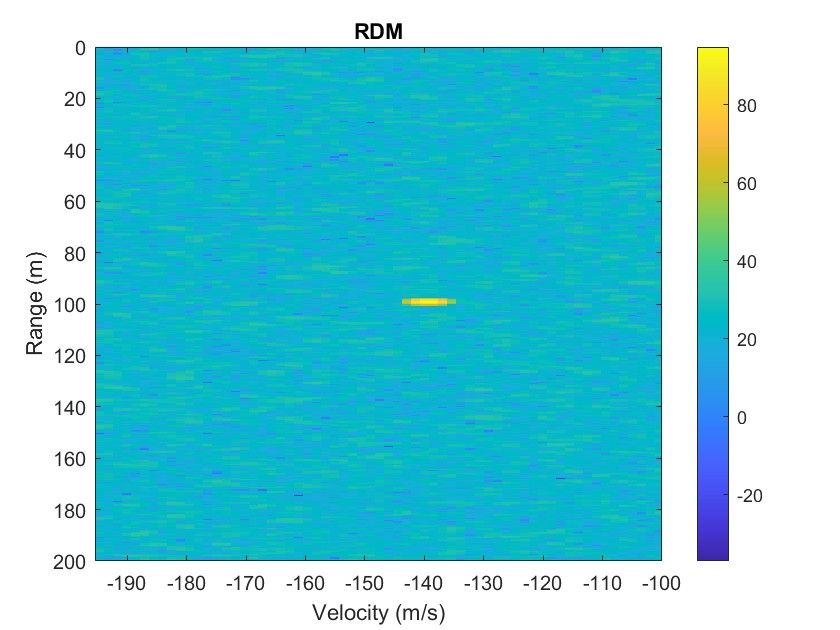
\includegraphics[width=0.8\linewidth]{ambig_velocity.jpg}}
	    	\caption{Range Doppler Matrix for Object at Ambiguous Velocity}
	    	\label{fig::ambig_velocity} 
	\end{figure}
	
	Figure \ref{fig::ambig_velocity} shows the RDM for this ambiguous velocity. The radar measures a velocity of -139.92 m/s. For an ideal system, the measured velocity can be computed as follows:
	
	\begin{equation}
		v_p = v\ \text{mod}\ 2v_{ua}
	\end{equation}
	
	\begin{equation}
		v_m = \begin{cases}
			v_p & 0 \leq v_p < v_{ua} \\
			v_p - 2v_{ua} & v_{ua} \leq v_p < 2v_{ua}
		\end{cases}
	\end{equation}
	
	Our measured velocity is consistent with this result.
	
	According to \cite{richards-2005}, the SNR at the receiver input is given by the following equation:
	
	\begin{equation}
		\chi = \frac{P_tG^2\lambda^2\sigma}{(4\pi)^3R^4kT_0\beta_nF_nL_sL_{\alpha}(R)}
	\end{equation}
	
	Each of the variables in the above expression are defined as follows:
	
	\begin{center}
	\begin{tabular}{|c|c|}
		\hline
		Variable & Definition \\
		\hline
		$P_t$ & Transmit Power \\
		\hline
		$G$ & Antenna Gain \\
		\hline
		$\lambda$ & Wavelength \\
		\hline
		$\sigma$ & RCS \\
		\hline
		$R$ & Distance to Object \\
		\hline
		$k$ & Boltzmann's Constant \\
		\hline
		$T_0$ & Temperature \\
		\hline
		$\beta_n$ & Noise Equivalent Bandwidth \\
		\hline
		$F_n$ & Noise Figure \\
		\hline
		$L_s$ & System Loss \\
		\hline
		$L_{\alpha}(R)$ & Atmospheric Loss \\
		\hline
	\end{tabular}
	\end{center}	
	
	If we consider only the contributions of the transmit power and noise equivalent bandwidth, we can derive the relationship among the remaining variables:
	
	\begin{equation}
		\chi \propto \frac{P_t}{\beta_n}
	\end{equation}
	
	Note that the SNR in the RDM is greater than the input SNR by a factor of $G_{sp}$, where $G_{sp}$ is the SNR gain due to signal processing. The signal processing gain for the FMCW radar is given by:
	
	\begin{equation}
		G_{sp} = G_{fast}G_{slow}
	\end{equation}
	
	Here, $G_{fast}$ is the SNR gain due to fast-time processing, and $G_{slow}$ is the SNR gain due to slow-time processing. The fast-time SNR gain is given as follows:
	
	\begin{equation}
		 G_{fast} = \frac{M_{fast}}{L_{fast}} = \frac{f_s/PRF}{L_{fast}}
	\end{equation}
		
	where $f_s$ is the sample rate and $L_{fast}$ is the SNR loss due to the fast-time FFT window. Using an 80 dB Chebyshev window, we get the following for $G_{fast}$:
	
	\begin{equation}
		G_{fast} \approx 860.8422
	\end{equation}
	
	Similarly, for the slow-time SNR gain, we have
	
	\begin{equation}
		G_{slow} = \frac{M_{slow}}{L_{slow}} = \frac{\#PRI}{L_{slow}}
	\end{equation}
		
	where $L_{slow}$ is the SNR loss due to the slow-time FFT window. Using an 80 dB Chebyshev window, we get the following solution for $G_{slow}$:
	
	\begin{equation}
		G_{slow} \approx 146.4771
	\end{equation}
	
	Therefore, the overall signal processing SNR gain is given by:
	
	\begin{equation}
		G_{sp} \approx 126094
	\end{equation}
	
	Or equivalently,
	
	\begin{equation}
		 {G_{sp}}_{(dB)} \approx 51.0069\ \text{dB}
	\end{equation}
	
	If we input a signal with an SNR of 20 dB and measure the SNR in the RDM, we obtain a value of 70.01 dB, which is consistent with the expected signal processing gain.
		
     \section {Communication (OFDM)}
     
	 \subsection {Background}
	 
	 	In this section, we provide background on OFDM (orthogonal frequency-division multiplexing). OFDM is a form of multicarrier modulation. In multicarrier modulation, the total channel bandwidth is divided into multiple subchannels, so that each subchannel experiences relatively flat fading. The subchannel spacing of OFDM differs from other forms of multicarrier modulation. OFDM modulates symbols on orthogonal subcarriers of the following form:
	 	
	 	\begin{equation}
	 		s_k(t) = e^{j2{\pi}kt/T_s}\text{rect}(t/T_s)
	 	\end{equation}
	 	
	 	where $T_s$ is the symbol duration.
	 	
	 	The orthogonality of the subcarriers allows the bandwidth of neighboring subchannels to be partially overlapped, improving spectral efficiency.
	 	
	 	A block diagram of an OFDM system is given in Figure \ref{fig::ofdm_block_diagram}.
		
	 	\begin{figure}[H]
	    		\centering
	    		\fbox{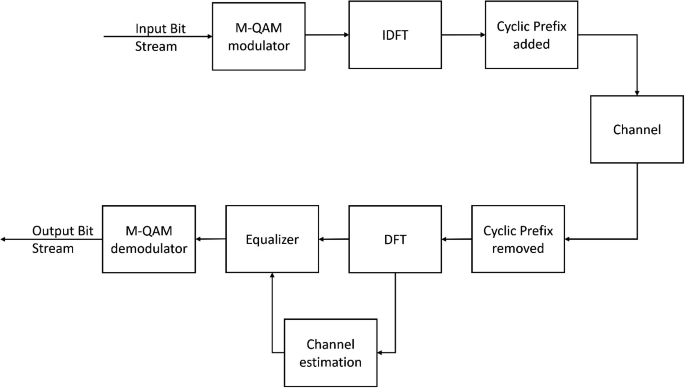
\includegraphics[width=0.9\linewidth]{OFDM Block diagram}}
	    		\caption{OFDM block diagram}
	    		\label{fig::ofdm_block_diagram}
		\end{figure}
		
		When a bit stream is received, it is modulated using the desired 2-D modulation scheme PSK, QAM, etc...). Then, it is placed into an FFT bin corresponding to a data subcarrier. Non-data carriers are reserved for pilot and null subcarriers as illustrated in Figure \ref{fig::ofdm_subcarriers}.
		
		\begin{figure}[H]
	    		\centering
	    		\fbox{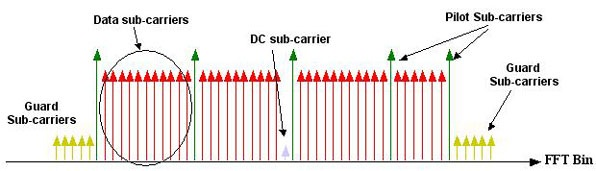
\includegraphics[width=0.9\linewidth]{OFDM subcarriers}}
	    		\caption{OFDM subcarriers}
	    		\label{fig::ofdm_subcarriers}
		\end{figure}
		
		Typically, null carriers are placed at the edges of the band to reduce interference between neighboring channels. A null carrier is also typically placed at DC to avoid problems with DC offsets in the D/A and A/D \cite{802_11a_standard}. An IFFT then modulates each of the symbols with its respective subcarrier.
		
		To deal with the effects of multi-path, a cyclic prefix is added to each of the OFDM symbols. The cyclic prefix appends the last L samples of an OFDM symbol to the beginning of the OFDM symbol as illustrated in Figure \ref{fig::cylic_prefix}.
		
		\begin{figure}[H]
	    		\centering
	    		\fbox{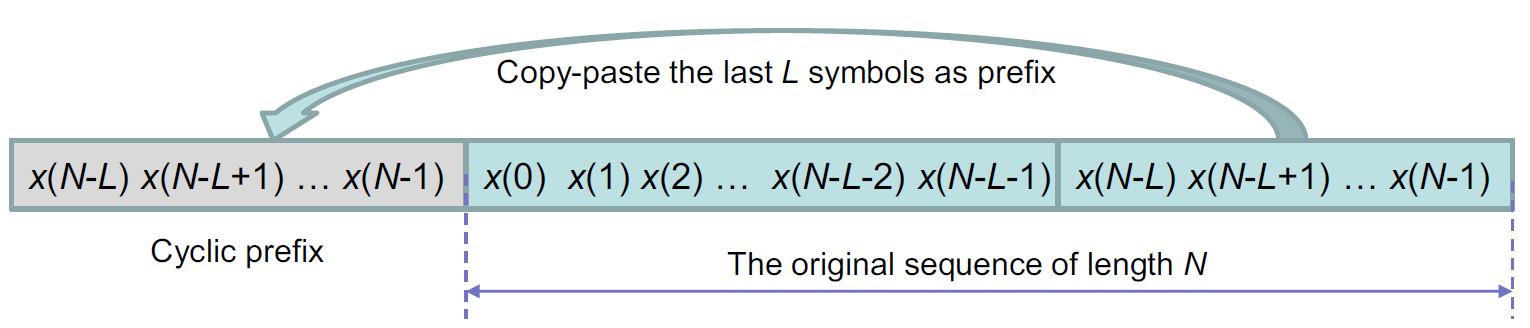
\includegraphics[width=0.9\linewidth]{cyclic_prefix.png}}
	    		\caption{OFDM Cyclic Prefix}
	    		\label{fig::cylic_prefix}
		\end{figure}
		
		At this stage, we can also add a window to reduce the out-of band spectrum. In the case of windowing, the first \newline $L/2 + L_{win}$ samples are appended to the end of the symbol and the last $L/2 + L_{win}$ samples are appended to the beginning of the symbol. This is illustrated in Figure \ref{fig::ofdm_windowing}.
		
		\begin{figure}[H]
	    		\centering
	    		\fbox{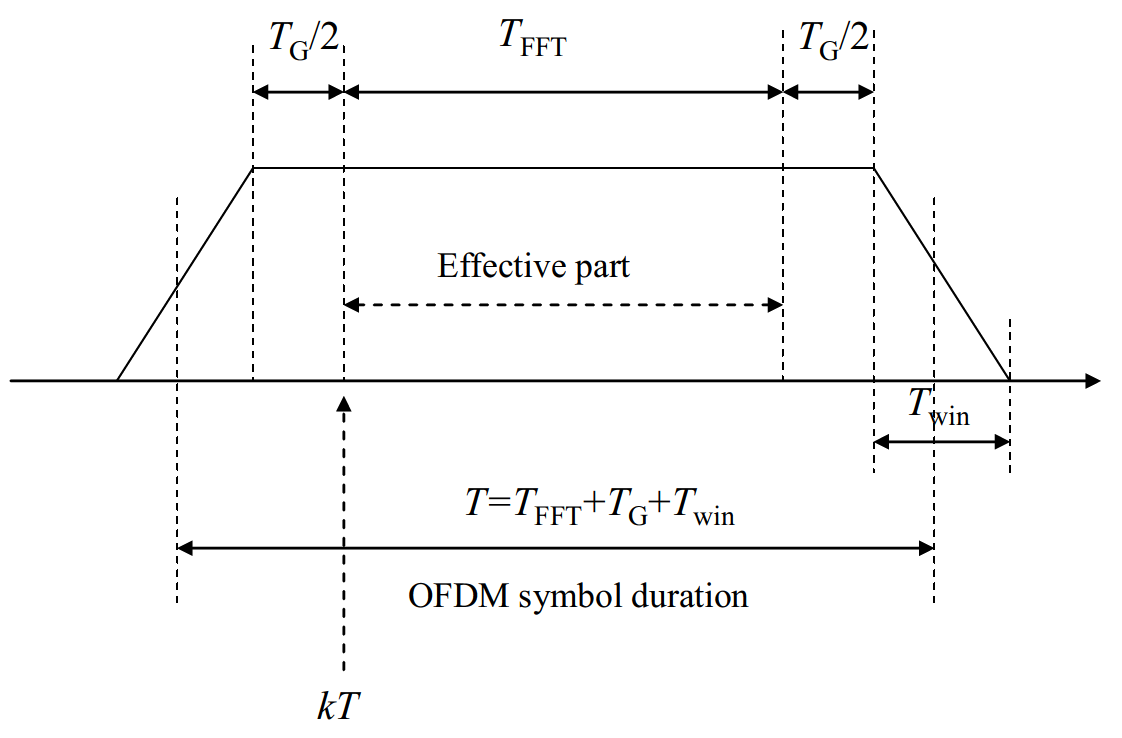
\includegraphics[width=0.9\linewidth]{ofdm_windowing.png}}
	    		\caption{OFDM Symbol with Windowing}
	    		\label{fig::ofdm_windowing}
		\end{figure}
		
		Then a window is multiplied element-wise with the symbol. A commonly applied window is
		
		\begin{equation}
			w_1(t) = \frac{1}{2}[1 - \cos\pi(t + T_{win} + T_G/2)/T_{win}]
		\end{equation}
		
		\begin{equation}
			w_2(t) = \frac{1}{2}[1 - \cos\pi(t - T_{FFT})/T_{win}]
		\end{equation}
		
		\begin{equation}
			w(t) = \begin{cases}
				w_1(t), & T_1 \leq t < T_2 \\
				1.0, & T_2 \leq t < T_3 \\
				w_2(t), & T_3 \leq t < T_4
			\end{cases}
		\end{equation}
		
		where $T_1$, $T_2$, $T_3$, and $T_4$ are defined as follows:
		
		\begin{equation}
			T_1 = -T_{win} - T_G/2
		\end{equation}
		
		\begin{equation}
			T_2 = -T_G/2
		\end{equation}
		
		\begin{equation}
			T_3 = T_{FFT} + T_G/2
		\end{equation}
		
		\begin{equation}
			T_4 = T_{FFT} + T_G/2 + T_{win}
		\end{equation}
		
		At the receiver, the window and or cyclic prefix are removed before the signal is demodulated with an FFT. Because of the cyclic prefix, each of the received multi-path components are a circularly-shifted copies of the transmitted signal. After the FFT, the multi-path components result in a complex weight for each of the FFT bins. We can remove this complex weighting by equalizing the received symbol. To perform equalization, we can estimate estimate the channel at each of the pilot carriers:
		
		\begin{equation}
			\hat{H}_{p_k} = \frac{Y_{p_k}}{X_{p_k}}
		\end{equation}
		
		We then can interpolate the channel estimate to get an estimate of the channel at each of the data carriers. Finally, we can compute equalization weights $A_k$ using either an zero-forcing or MMSE equalizer.
		
		\begin{equation}
			A_{\text{ZF}_k} = \frac{1}{\hat{H}_k}
		\end{equation}
		
		\begin{equation}
			A_{\text{MMSE}_k} = \frac{\hat{H}_k^{*}}{|\hat{H}_k|^2 + 1/SNR}
		\end{equation}
		
		After equalization, we should be obtain to correctly reconstruct the symbols contained in the OFDM data carriers. Each of these symbols can then be demodulated to obtain the resulting bit stream.		
		
		
		
		 can be computed based on the  each of the data carriers.  
		 		
		First, a bit-stream is modulated using a desired modulation (PSK, QAM, etc...)
	 	
	 	
	 	We specifically concentrate on the 802.11p standard, which is designed specifically for V2V communication. The 802.11p described in \cite{802_11p_abdelgader}
	 	
	     In this section we skim through OFDM communicaiton protocol. Since the objective of this paper is V2V JRC our focus is on IEEE 802.11 P standard. In this section we familiarize ourself with the functionality, key features, some 802.11 P standard specificaitons and advantages of this communication topology.\par
    \textbf{  802.11 P} is specifically designed for wireless access in vehicular environments (WAVE) and is widely used for V2V applications within the automotive industry.
      
      \begin{itemize}
      \item Frequency Band:		5.850 GHz to 5.925 GHz (DSRC Band)
	\item Channel Bandwidth:	10 MHz
	\item Modulation:		BPSK, QPSK, 16-QAM
	\item Maximum Data Rate:	27 Mbps (Theoretical)
	\item Range: 			Up to 1 km (ideal conditions)
	\item Vehicle Speed :                Up to 200 km/h
	\item Security:			WPA2, Authentication, Message Integrity
	\item Applications:		Collision avoidance, traffic management, V2X
	\end{itemize}
	
 \textbf{ Orthogonal Frequency Division Multiplexing (OFDM)} is widely used in Vehicle-to-Vehicle (V2V) communication systems for several reasons, including inherent characteristics that provide efficient data transmission in dynamic, high-speed environments.

Block diagram below is a typical OFDM process from input bit steam, modulation, through the channel, DFT, demodulation and output bit steam. 
      
      The graph below illustrat a typical OFDM fram (64-subcarrier example)
      
      	\begin{itemize}
      	\item Guard Band (Zero Subcarriers): Subcarriers 0–5 and 59–63
	\item Data Subcarriers: Subcarriers 6–28 and 37–58
	\item Pilot Subcarriers: Subcarriers 7, 21, 43, 57
	\item DC Subcarrier (Zero): Subcarrier 32
	\end{itemize}
		
Some of OFDM's perform metrics of interest that we are going to analize in this paper include but are not limited to:

\begin{itemize}
\item Received SNR
\item Bit Error Rate (BER)
\item Channel Capacity
\end{itemize}

One channel's property needs to be analysed and compared is the channel capacity. We use the simple fromula below (Shannon-Hartley theorem) to calculate the channel capacity. 
Where Bk is the bandwidth of the k-th subcarrier, Pk, transmit power, Hk, frequency response magnitude and Nk is a noise power.   
%Where H (m, n) , Hmn is the channel frequency response of the n symbol on the m sub carrier. 
	
		%\begin{equation}
		%	    		C_{m,n} = \text{log}_2\left(1 + \text{SNR}|H(m,n)|^2\right)
	    	%	\label{eq:ofdm_capacity}
		%\end{equation}

			\begin{equation}
			C_{k} = B_{k}.\text{log}_2\left(1 +\frac{ \text P_{k}.|H_{k}|^2}{N_{k}}\right)
	    		\label{eq:ofdm_capacity}
	    		\end{equation}

\subsection {Simulation and Performance}
      
      We have developed comprehensive MATLAB code to evaluate the performance of an OFDM communication system. Metrics of interest include the peak to average power ratio (PAPR), the bit error rate (BER) in an AWGN channel, the BER in presence of Rayleigh fading, and the capacity of the system.
      
      For this analysis, we chose to evaluate an OFDM 802.11p system because the 802.11p standard is applicable to VNV communication \cite{802_11p_abdelgader}. The 802.11p standard operates in the DRC Band (5.850 GHz to 5.925 GHz) and uses 64 subcarriers sampled at a rate of 10 MHz. A 16 sample cyclic prefix is added, increasing the symbol duration from 6.4 ${\mu}s$ to 8.0 ${\mu}s$. Of the 64 subcarriers, 48 are data carriers, and 4 are pilots. Pilots are specifically located at $\{-21, -7, 7, 21\}$. Data carriers cover all the remaining carriers in range $[-26, 26]$ except the DC subcarrier, which is a null carrier.
      
    The power spectral density of the transmitted OFDM signal is shown in Figure \ref{fig::ofdm_psd}.
    
    \begin{figure}[H]
    		\centering
    		\fbox{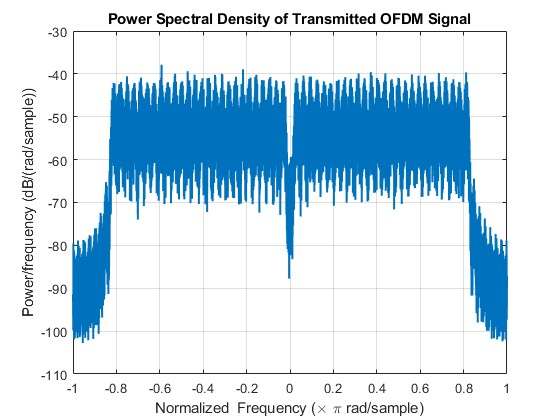
\includegraphics[width=0.8\linewidth]{OFDM Power spectral density}}
    		\caption{OFDM Power Spectral Density}
    		\label{fig::ofdm_psd}
	\end{figure}
    
    The location of null carrier is also consistent with the 802.11p standard. We were able to perform power measurements on this signal to determine the PAPR. When the data carriers are modulated using QPSK modulation, we measure a PAPR of 11.8 dB. The measured PAPR is significant because it forces us to run the high power amplifier at reduced power levels, which can degrade the transmitted power and in turn the SNR of the system.
    
    To evaluate the BER in an AWGN channel, we add gaussian noise to the transmitted signal to achieve a given SNR. Then, we process the resulting signal with a model of the OFDM receiver. After FFT processing, we can generate a constellation diagram from the resulting data carriers. Figure \ref{fig::rx_constellation_diagram} shows the received constellation diagram for an OFDM signal using QPSK modulation at 20 dB SNR.
      
      \begin{figure}[H]
		\centering
    		\fbox{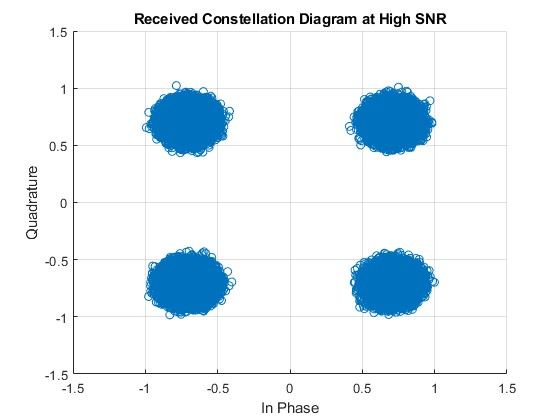
\includegraphics[width=0.8\linewidth]{OFDM AWGN Constellation}}
    		\caption{OFDM Received Constellation after AWGN Channel}
    		\label{fig::rx_constellation_diagram}
  	  \end{figure}
    
    		The expected bit error rate (BER) for a single OFDM subcarrier is identical to the BER of a single carrier system, when the SNR of the given subcarrier is considered. For QPSK, this is approximately given by
		
		\begin{equation}
			P_b(\rho_b) \approx Q(\sqrt{2\rho_b})
		\end{equation}
		
		where $\rho_b$ is the SNR per bit. If the modulation is the same for each OFDM subcarrier, the BER is the mean BER for all active data carriers. In Figure \ref{fig::ofdm_awgn_ber}, we examine the BER of an OFDM system vs SNR.
		
		\begin{figure}[H]
			\centering
    			\fbox{\includegraphics[width=0.8\linewidth]{OFDM AWGN BER vs SNR}}
    			\caption{OFDM BER vs. SNR in AWGN channel}
    			\label{fig::ofdm_awgn_ber}
		\end{figure}
		
		The SNR of each active subcarrier is 64/52 times (or 0.9018 dB) greater that of the received signal because all the signal energy is concentrated in the active subcarriers. After accounting for this SNR gain, the resulting BER is equivalent to the expected BER. 
        
        We also examine the BER of the OFDM receiver in the presence of Rayleigh fading. To do so, we apply Rayleigh fading to the signal amplitude prior to applying additive white gaussian noise. We can then generate a received constellation map for each of the symbols modulated on the data carriers. For 20 dB SNR, the received constellation map is shown in Figure \ref{fig::ofdm_rayleigh_fading}.
        
      \begin{figure}[H]
		\centering
    		\fbox{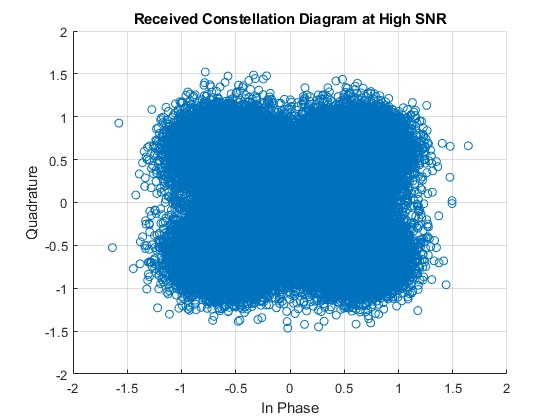
\includegraphics[width=0.8\linewidth]{OFDM Constellation Diagram}}
    		\caption{OFDM Received Constellation Diagram after Rayleigh Fading}
    		\label{fig::ofdm_rayleigh_fading}
  	  \end{figure}
    
    		We can compare the received constellation to the one shown in Figure \ref{fig::rx_constellation_diagram}. Doing so, we observe that the clusters are not easily separable like they were previously, indicating a much higher BER. The average BER in the presence of fading can be computed as follows:
    		
    		\begin{equation}
    			\bar{P}_b = \int_{0}^{\infty}{P_b(\rho)f(\rho)d\rho}
    		\end{equation}
    		
    		$f(\rho)$ is the distribution of the SNR due to Rayleigh fading and is given by
    		
    		\begin{equation}
    			f(\rho) = \frac{1}{\bar{\rho}}e^{-\frac{\rho}{\bar{\rho}}}
    		\end{equation}
    			
    		where $\bar{\rho}$ is the average SNR. In Figure \ref{fig::ofdm_fading_ber}, the measured BER in the presence of Rayleigh fading is compared to the expected BER.
    		
    		\begin{figure}[H]
			\centering
    			\fbox{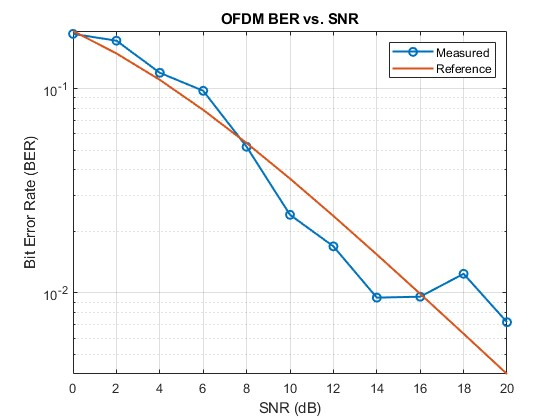
\includegraphics[width=0.8\linewidth]{OFDM BER vs SNR}}
    			\caption{OFDM BER vs. SNR in Rayleigh Fading}
    			\label{fig::ofdm_fading_ber}
  	  	\end{figure}
  	  
  	  	Referring to the figure, the measured BER rate is consistent with the expected BER.
    		
    		
    		can compare the results to the results shown in Figure 15.
    For our To evaluate the performance of the 802.11p system, we generated OFDM symbols and fed them through a channel model and into an simulated OFDM receiver. The power spectral density of the transmitted signal using QPSK is shown below:
      
    \begin{figure}[H]
    		\centering
    		\fbox{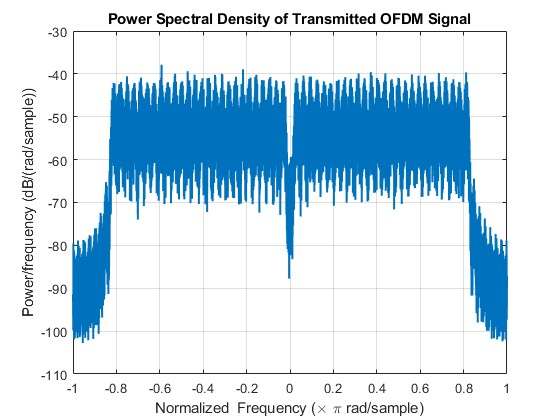
\includegraphics[width=0.8\linewidth]{OFDM Power spectral density}}
    		\caption{OFDM Power Spectral Density}
	\end{figure}
      
      To evaluate the peak-to-average power ratio, we generated OFDM symbols using QPSK to modulate each of the data carriers. We then measured the ratio of peak to average power to be roughly 11.8 dB.  The resulting spectrum from our simulation is shown below:
      
      
       pFor the simulations that follow, we use QPSK modulation to encode each of the data subcarriers.
      
	  
		
		After accounting for an SNR increase of $64/52$ due to the signal power being concentrated in the data subcarriers.
				
		The SNR of an individual subcarrier is $64/52 \times$ that of the received signal because the . 
		
		The SNR After accounting for the increase an increase in SNR of 64/52 due to coherent gain on 52 of the 64 subcarriers
	
	
       and plot the Bit Error Rate (BER) versus SNR across various channel conditions.. Evaluating diverse channel characteristics is key to achieving a comprehensive and unbiased analysis in our study. The summary implemntation of a complete OFDM simulation model parameters and results for AWGN, Rayleight Fading and perfect channel provided below. 
      
\begin{itemize}
\item 64 Subcarriers, 48 Data carriers, 10 K Symbols adn 16 Cyclic-prefix
\item 4th order QAM modulation and 10 MHz Sample rate
\item Pilots are inserted at standard intervals and zero carriers are placed at the edges of the spectrum.
\item The IFFT converts the frequency domain symbols to the time domain. 
\item A Hamming window is applied to each OFDM symbol to reduce spectral leakage. 
\item A cyclic prefix is added to the windowed OFDM symbols to mitigate ISI. 
\item An AWGN channel is used to transmit the flattened signal to the receiver.\par
\item The receiver removes the cyclic prefix. 
\item The data sub-carriers are extracted and demodulated from FFT, results in frequency domain. 
\item The received bits are compared to the transmitted bits to calculate the BER vs SNR values. 
\end{itemize}
The power spectral density of trasmitted OfDM signal shown in the graph below. The flat region conrresponds to the active subcarriers of the OFDM signal (each subcarrier carries equal power and spans the same bandwidth). There is a dip null in the center correspoinding to the DC (zero frequency) subcarrier which used to avoid interference. The dips at the edges are the guard bands to rduce spectral leakage and interference with adjacent channels.

	\begin{figure}[H]
    		\centering
    		\fbox{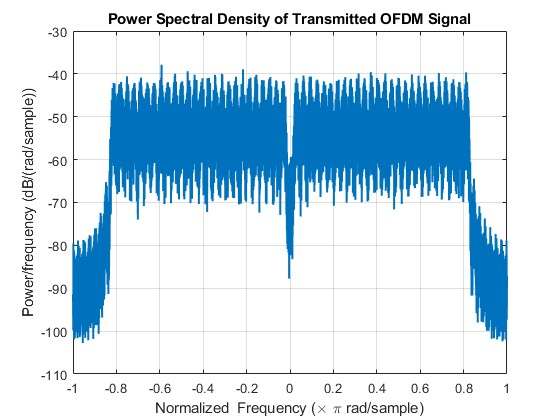
\includegraphics[width=0.8\linewidth]{OFDM Power spectral density}}
    		\caption{OFDM Power Spectral Density}
	\end{figure}

  The graph below is a constellation coresponding to 4th order QAM with AWGN channel propery.  The points are tightly packed around the ideal constellation locations, indicating that noise has minimal impact on the received signal (high SNR conditions).This diagram demonstrates that the system performs well under high SNR conditions, maintaining accurate symbol transmission and reception.
    
    
     
    
    The BER decreases exponentially as the SNR increases, which is typical for digital communication systems. The close alignment of the measured and reference curves validates the simulation accuracy and ensures the OFDM system is working as intended. The system shows robust performance at higher SNR values, achieving nearly error-free communication. This analysis is crucial for validating the system and ensuring its effectiveness in real-world applications.
    
    
         \begin{figure}[H]
		\centering
    		\fbox{\includegraphics[width=0.8\linewidth]{OFDM AWGN BER vs SNR}}
    		\caption{OFDM BER vs. SNR (AWGN) }
  	  \end{figure}
    

  The results below are from the same signal charactristics transmitted through Rayleigh fading channel. The points are tightly clustered around the ideal constellation positions (caused by delay fading) that implying effective channel conditions and robust equalization process. The constellation diagram results indicates that the system operates in a highl SNR environment where noise has minimal impact. 

	\begin{figure}[H]
		\centering
    		\fbox{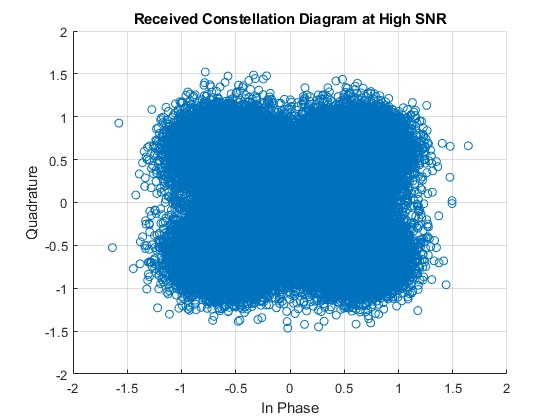
\includegraphics[width=0.8\linewidth]{OFDM Constellation Diagram}}
    		\caption{OFDM Constellation Diagram  (Rayleigh)}
  	  \end{figure}

The plot below represents the Bit Error Rate (BER) vs. Signal-to-Noise Ratio (SNR) performance of an OFDM system. It compares the measured BER from the simulation against the theoretical (reference) BER for the given modulation scheme and channel model. Both curves show a monotonic decrease in BER with increasing SNR, which is expected as higher SNR improves the signal quality and reduces errors. Around 6-10 dB, the curve begins to drop sharply, indicating the SNR threshold beyond which the system transitions from error-prone to error-free performance. This plot confirms that the OFDM system performs reliably under high SNR and aligns closely with theoretical predictions.
    
    \begin{figure}[H]
		\centering
    		\fbox{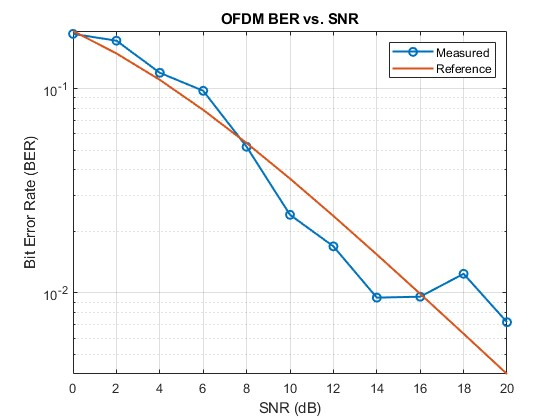
\includegraphics[width=0.8\linewidth]{OFDM BER vs SNR}}
    		\caption{OFDM BER vs. SNR}
  	  \end{figure}    
  	  
  	  For the given parameter, B total=10 MHz, N subcarriers=64, N data=48, P total =1 W (assumed for simplicity) and No=1 nW/Hz, the total channels capacity for given OFDM  with AWGN is around 99.74 Mbps. \par
  	 It is important to highlight the cyclic prefix reduces the effective data rate, which slightly decreases the channel capacity. Adjust for this overhead if needed.
 
  	  
    
    \section {JRC}
		 \subsection {Background}
		 
 The convergence of radar and communication systems, often referred to as joint radar-communication (JRC), has emerged due to several technological and practical motivations. Some of the primary reasons why radar and communication systems are being integrated listed below :
 
 \begin{itemize}
 \item Spectrum Sharing adn Efficiency (coexisting within the same frequency band)
\item Shared Hardware
\item Autonomous Vehicles
\item Energy Efficiency		 
\end{itemize}		 
		 
The orthogonality or low correlation of the frequency domain allows the two subsystems not to interfere with each other. The disadvantage is that the spectrumutilization of the system is low and energy sharing is difficult to achieve. Other crutial disadvantage we need to overcome is OFDM signals are sensitive to the Doppler shift and multipath effects, which leads to a loss of subcarrier orthogonality and intersymbol interference (ISI) \cite{9992221}.

\subsection {Simulation and Performance}
      
There are many variables and parameters that can influence the quality of the received data. To investigate the accuracy of the JRC received data, we have simulated and compared the results for many scenarios. The first OFDM-Radar simulation consists of DC subcarrier (Zero Frequency) which is used in OFDM signals to avoid issues with DC offset in the receiver, eliminate interference from low-frequency noise. 

\begin{figure}[H]
\centering
\fbox{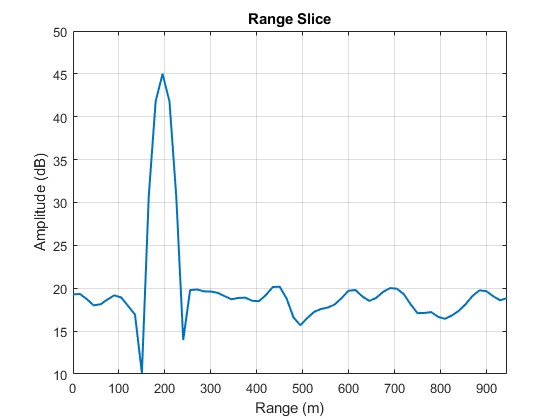
\includegraphics[width=0.8\linewidth]{OFDMRadar_with DCNull_200m}}
\caption{OFDM/Radar with DC null range plot}
\end{figure}

The next plot displays the signal with the same parameter without the DC null. The pick received power is almost the same as the signal received with DC null. However, the sidelobes and noise floor shifted down significantly (average of 17 dB lower). Lower sidelobes and noise floor is crucial to some applications with high scattering noise. By including DC offset, the available bandwidth is fully utilized, leading to better spectral efficiency. Each subcarrier contributes to the total system data rate. Utilizing the DC subcarrier adds additional capacity, increasing the total throughput of the system.

\begin{figure}[H]
\centering
\fbox{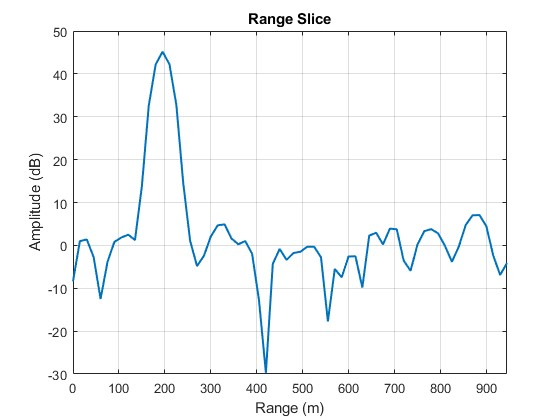
\includegraphics[width=0.8\linewidth]{OFDMRadar_No DCNull_200m}}
\caption{OFDM/Radar without DC null range plot}
\end{figure}

The previous results were simulated for a target located at 200m. We have increased the target range to 500 and 1000m to see the received data quality and degradation in a long target range. As the plots indicate, in the 500m range which considers a long range for V2V radar applications, we still have a distinguishable target peak (delta of 23dB). At 900m range the dynamic range degrades significantly to around 9dB. \par
\textbf{ Note: } To have an efficient report, we only display the analysis for signals without the DC Nulls.
\begin{figure}[H]
\centering
\fbox{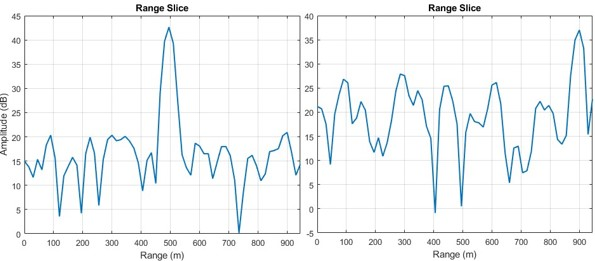
\includegraphics[width=1.0\linewidth]{Mix_500-900m}}
\caption{OFDM/Radar No DC null range plot 500m (left) and 900m (right)}
\end{figure} 
Doppler is one other critical parameter to identify the reliable radar system. The Doppler simulation results provided for both 500 and 900m in the figure below. As we expected the higher range degrades the Doppler results dynamic range (22 to 14 dB). However, in this Doppler result the resolution is not adequate to provide an accurate result. The flat signal peak indicates a high ambiguity and unreliable target velocity estimation.
\begin{figure}[H]
\centering
\fbox{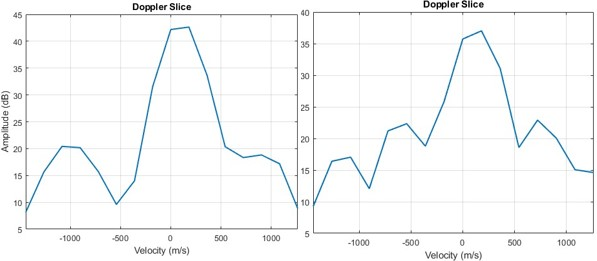
\includegraphics[width=1.0\linewidth]{Mix_500-900m_Doppler}}
\caption{OFDM/Radar Doppler plot for 500m (left) and 900m (right)}
\end{figure} 

A key advantage of the OFDM technique is its flexibility to adjust parameters, enabling optimal performance tailored to the application and channel characteristics in various environments. We have adjusted the OFDM parameters to optimize radar performance while preserving high communication efficiency and capacity.
OFDM radar written in MATLAB and configured with the following set of parameters: 

\begin{center}
\begin{tabular}{|c|c|}
\hline
\textbf {Parameter} & \textbf {Value }\\
\hline
Carrier Frequency & 77 GHz \\
\hline
Sample Rate & 200 MHz \\
\hline
Number of Subcarriers & 16x64\\
\hline
Number of Data Carriers & 16x48 + 1 \\
\hline 
Number of Pilot Carriers & 16x4 \\
\hline 
Number of Pulses & 128 \\
\hline 
Target Range & 200 \\
\hline 
Target Velocity & 50 \\
\hline 
\end{tabular}
\end{center}


The graph below presents the simulation results using the parameters described above. While the noise floor has risen to 45 dB, the dynamic range remains around 38 dB, similar to the unimproved simulation at a 200m range. Another significant improvement is the enhanced resolution of the detected peak, leading to more accurate range measurements.

\begin{figure}[H]
\centering
\fbox{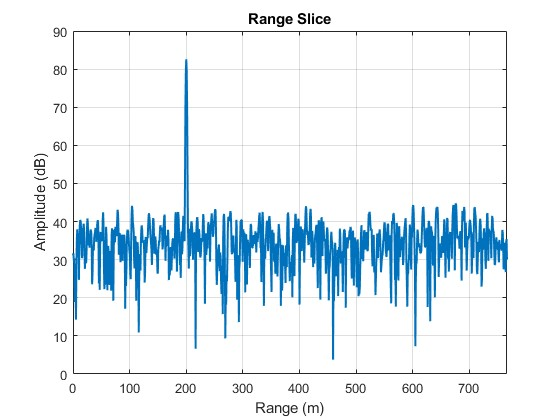
\includegraphics[width=0.8\linewidth]{OFDMRadar_No DCNull_T200_Improve}}
\caption{OFDM/Radar range plot for 200m target}
\end{figure} 
The Doppler results for the above parameters plotted in the graph below. 
\begin{figure}[H]
\centering
\fbox{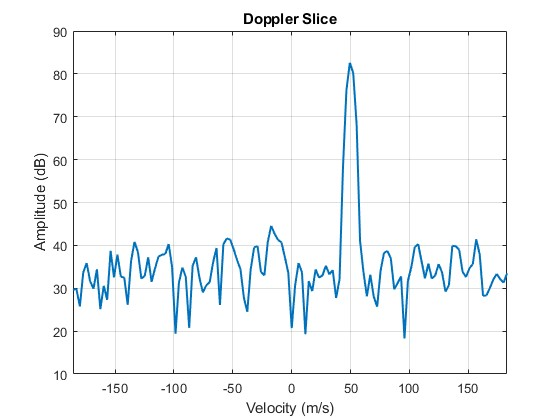
\includegraphics[width=0.8\linewidth]{OFDMRadar_No DCNull_Doppler_T200_Improve}}
\caption{OFDM/Radar range plot for 200m target}
\end{figure} 
Finally, we present the maximum achievable range with sufficient resolution to facilitate easy target analysis and detection. The best results were achieved at 700m. The received signal degraded significantly after 700m range. 

\begin{figure}[H]
\centering
\fbox{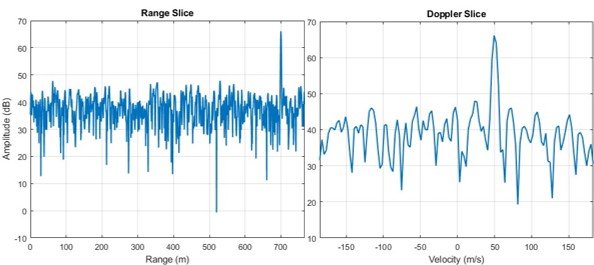
\includegraphics[width=0.8\linewidth]{Mix_Improved_700m}}
\caption{OFDM/Radar range (left) and Doppler (right) plot for 700m target}
\end{figure} 
\section {Conclusion}
While JRC may slightly compromise the standalone performance of either radar (resolution) or communication (capacity), it offers significant advantages in shared resource utilization, reduced hardware cost, and suitability for modern multi-functional systems like autonomous vehicles.


	\bibliographystyle {IEEEtran}
	\bibliography {References}
	
	%\nocite{yang_subcarrier_multiplexing}
	%\bibliography{sources}{}
   % \bibliographystyle{ieeetr}
  
\end{document}

